\documentclass{article}

\usepackage{graphicx}
\usepackage{tikz}
\usepackage{tikzsymbols}
\usetikzlibrary{calc,patterns,shapes.geometric}
\pagestyle{empty}
\usepackage[margin=0pt]{geometry}
\geometry{papersize={14in,12in}}

\def\centerarc[#1](#2)(#3:#4:#5){\draw[#1] ($(#2)+({#5*cos(#3)},{#5*sin(#3)})$) arc (#3:#4:#5);}

\begin{document}
	\begin{figure}
		\centering
		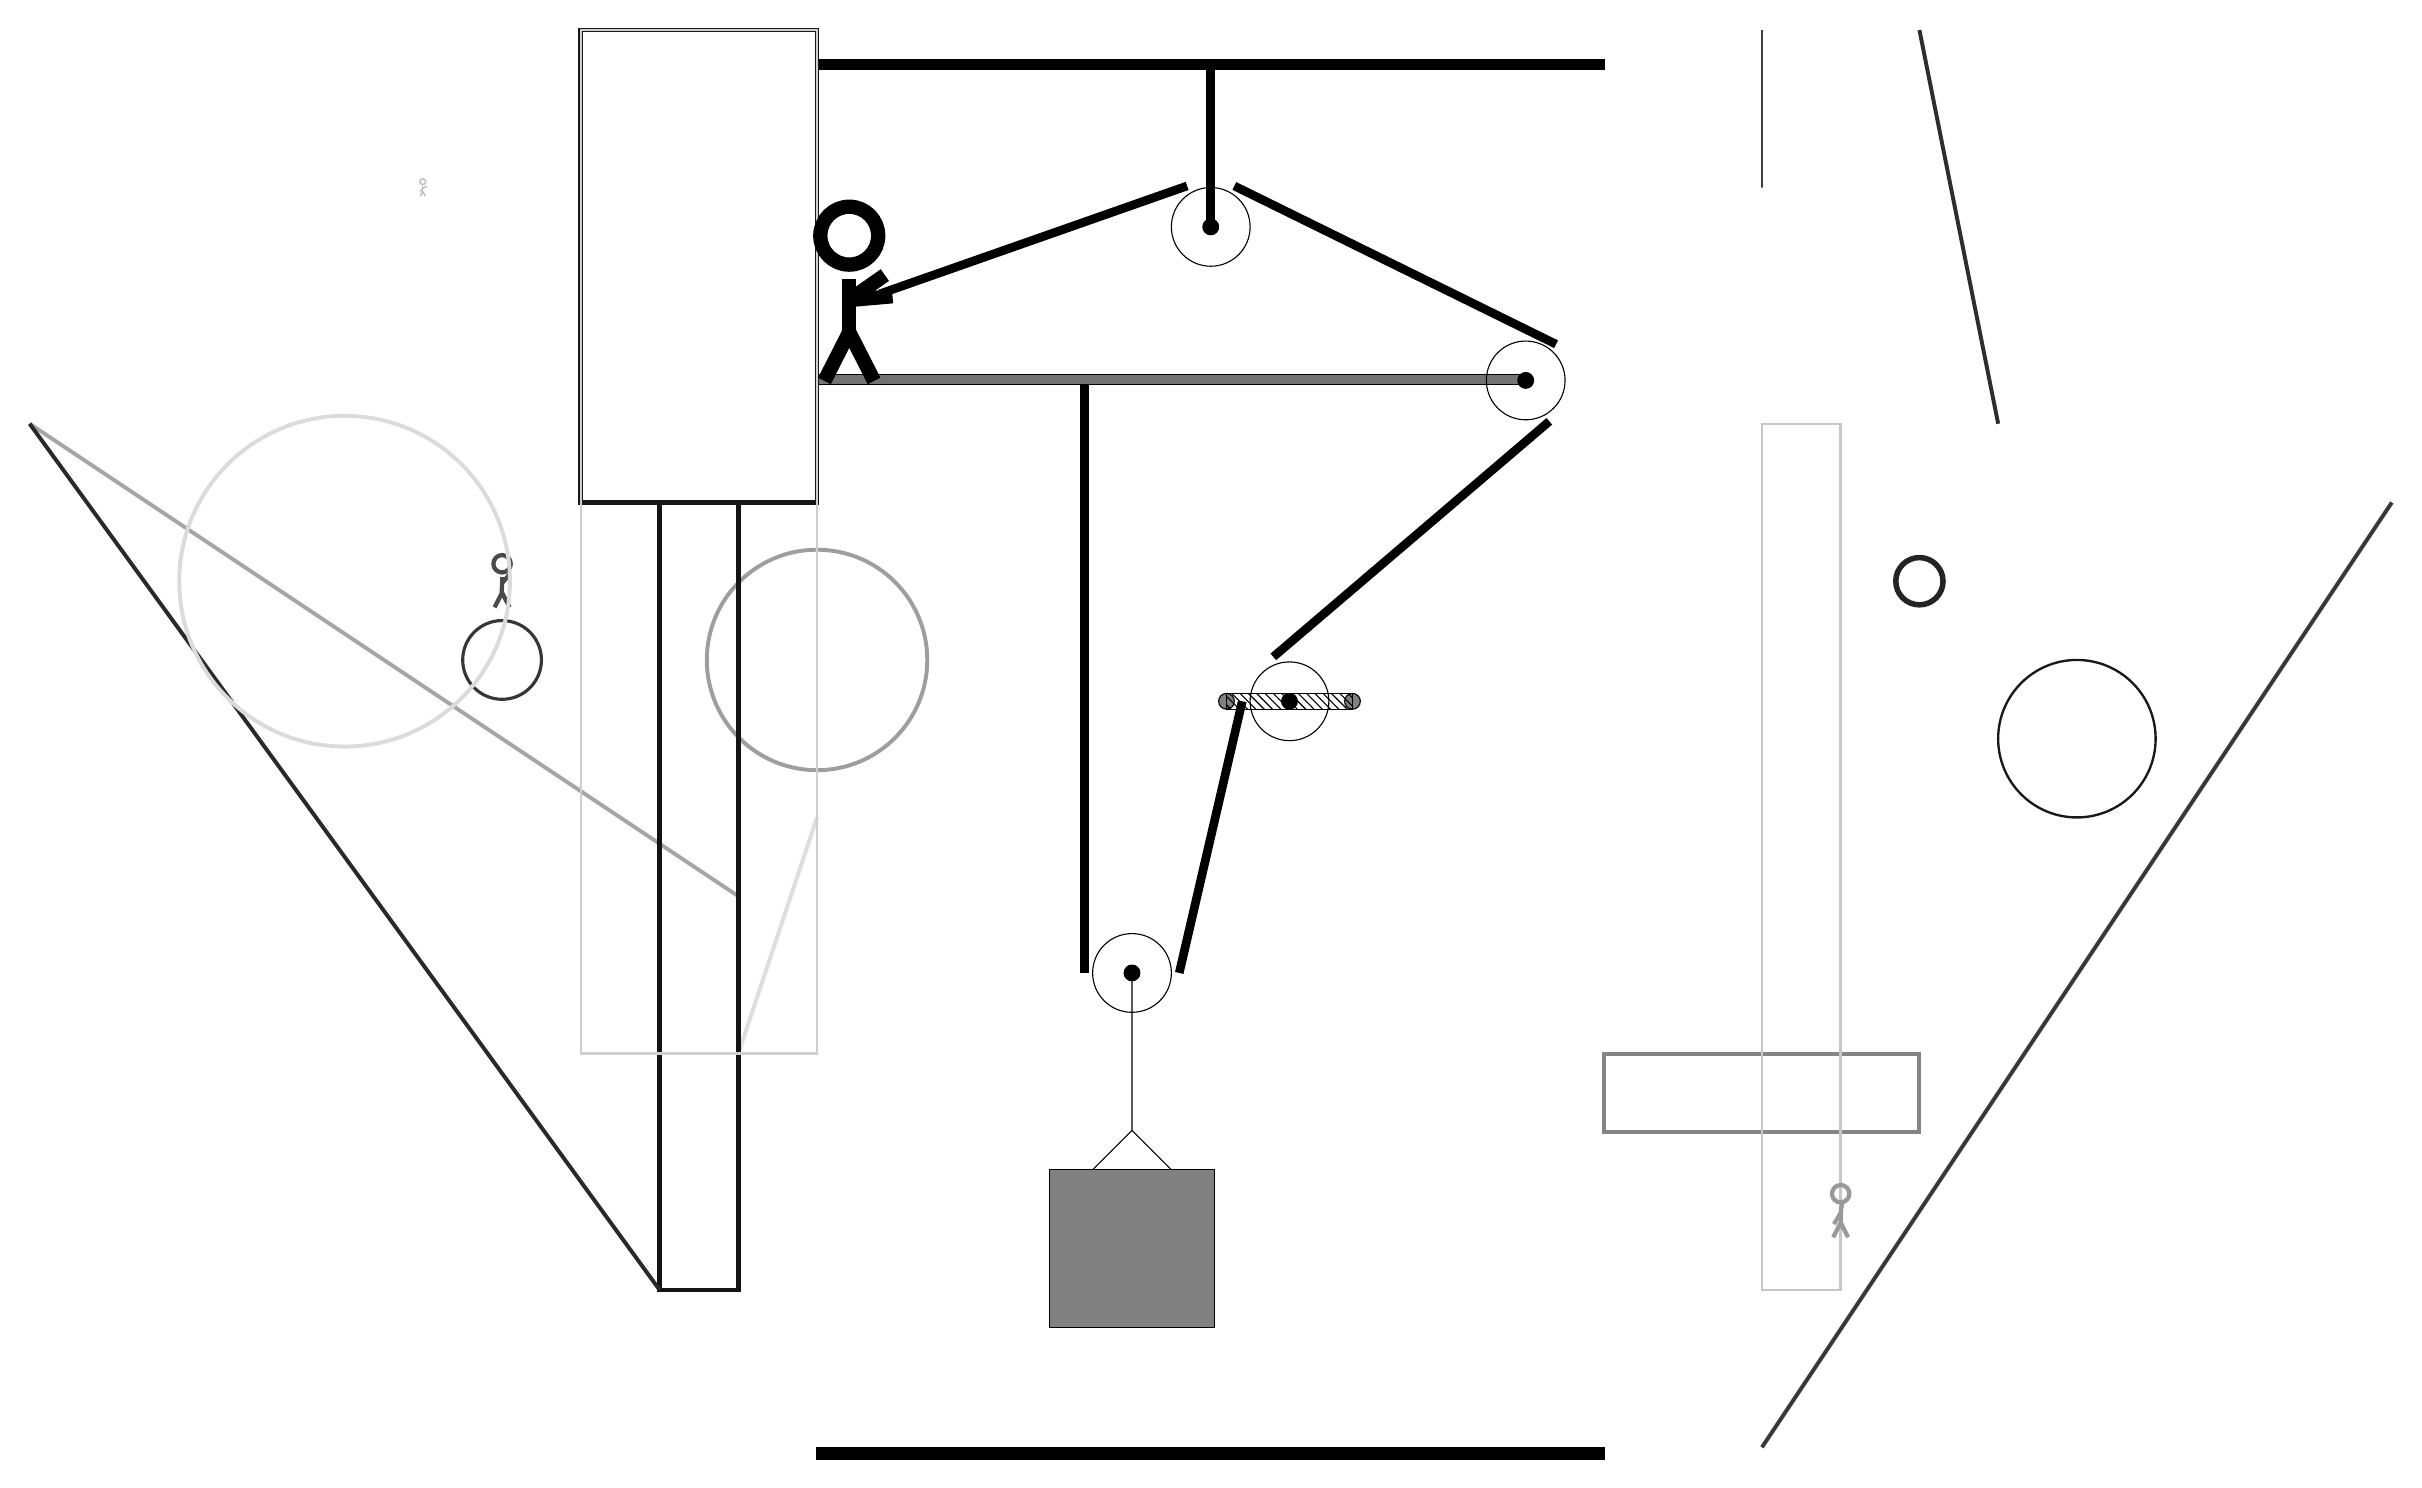
\begin{tikzpicture}
			%%%%% START %%%%%
			
			\draw[fill=black] (-2, 15.5) rectangle (8, 15.625);
			
			\draw[fill=black!55] (-2, 11.5) rectangle (7, 11.625);
			
			\draw (2, 4.025) circle (0.5);
			\draw[fill=black] (2, 4.025) circle (0.1);
			
			\draw[line width=0.5mm, color=black!82](12, 16) -- (13, 11);
			
			\draw [line width=0.5mm, color=black!38](-2, 8) circle (1.4);
			\draw[line width=0.5mm, color=black!48] (8, 2) rectangle (12, 3);
			\draw[line width=0.5mm, color=black!13](-3, 3) -- (-2, 6);
			
			\draw[line width=0.3mm, color=black!22] (10, 11) rectangle (11, 0);
			\node[line width=0.4mm, color=black!40] at (11, 1) {\Strichmaxerl[3][59][82]};
			\draw[line width=0.5mm, color=black!35](-3, 5) -- (-12, 11);
			\draw [line width=0.7mm, color=black!86](12, 9) circle (0.3);
			\draw[line width=0.6mm, color=black!92] (-3, 0) rectangle (-4, 10);
			\draw[line width=0.5mm, color=black!84](-4, 0) -- (-12, 11);
			
			\draw [line width=0.4mm, color=black!79](-6, 8) circle (0.5);
			\draw[line width=0.2mm, color=black!76] (10, 16) rectangle (10, 14);
			\draw[line width=0.6mm, color=black!91] (-2, 16) rectangle (-5, 10);
			\draw [line width=0.3mm, color=black!90](14, 7) circle (1.0);
			\node[line width=0.6mm, color=black!26] at (-7, 14) {\Strichmaxerl[1][51][22]};
			\node[line width=0.6mm, color=black!71] at (-6, 9) {\Strichmaxerl[3][88][49]};
			
			\draw[line width=0.3mm, color=black!19] (-2, 16) rectangle (-5, 3);
			\draw[line width=0.5mm, color=black!78](10, -2) -- (18, 10);
			\draw [line width=0.5mm, color=black!14](-8, 9) circle (2.1);
			
			\draw (7, 11.55) circle (0.5);
			\draw[fill=black] (7, 11.55) circle (0.1);
			
			\draw[fill=white](4, 7.475) circle (0.5);
			\draw[fill=black] (4, 7.475) circle (0.1);
			\draw[fill=black!50] (3.2, 7.475) circle (0.1);
			\draw[fill=black!50] (4.8, 7.475) circle (0.1);
			\draw[pattern=north west lines, pattern color=black] (3.2, 7.575) rectangle (4.8, 7.375);
			
			\draw (3, 13.5) circle (0.5);
			\draw[fill=black] (3, 13.5) circle (0.1);
			\draw[line width=1.1mm] (3, 13.5) -- (3, 15.5);
			
			\draw (2, 4.025) -- (2, 2.025) -- (1.5, 1.525) -- (2.5, 1.525) -- (2, 2.025);
			\draw[fill=black!50] (0.95, 1.525) rectangle (3.05, -0.475);
			
			\draw[line width=1.1mm] (1.4, 11.5) -- (1.4, 4.025);
			\centerarc[line width=1.1mm](2, 4.025)(180:360:0.6);
			\draw[line width=1.1mm](2.6, 4.025) -- (3.4, 7.475);
			\centerarc[line width=1.1mm](4, 7.475)(110:180:0.6);
			\draw[line width=1.1mm](3.7948, 8.0388) -- (7.3, 11.0304);
			\centerarc[line width=1.1mm](7, 11.55)(-60:50:0.6);
			\draw[line width=1.1mm](7.3857, 12.0096) -- (3.3, 14.0196);
			\centerarc[line width=1.1mm](3, 13.5)(60:120:0.6);
			\draw[line width=1.1mm](2.7, 14.0196) -- (-1.2, 12.65);
			
			\node at (-1.5, 12.65) {\Strichmaxerl[10][-175][35]};
			
			\draw[fill=black] (-2, -2) rectangle (8, -2.15);
			
			%%%%% END %%%%%
		\end{tikzpicture}
	\end{figure}	
\end{document}